
%\section{PHÉP CHIA ĐA THỨC VÀ BÀI TOÁN THỰC TẾ} % Tên bài
\subsection{Chia một đơn thức cho một đơn thức}
\subsubsection{Kiến thức trọng tâm}
\begin{tomtat}
	\begin{itemize}
		\item 
		Đơn thức $A$ chia hết cho đơn thức $B$ khi mỗi biến của $B$ đều là biến của $A$ với số mũ của $B$ không lớn hơn số mũ của $A$.
		\item Muốn chia đơn thức $A$ cho đơn thức $B$ (trong trường hợp chia hết) ta làm như sau:
		\begin{itemize}
			\item Chia hệ số của $A$ cho hệ số của $B$.
			\item Chia từng biến trong $A$ cho từng biến đó trong $B$.
			\item Nhân các kết quả vừa tìm được với nhau.
		\end{itemize}
	\end{itemize}
\end{tomtat}

\begin{vd}%[Dự án EX-9-Đề Cương Toán 8]%[Nguyễn Chiến]%[8D1H2-4]
	Tính
	\begin{multicols}{2}
		\begin{enumerate}
			\item $12x^6y:(-4x^2y)$; 
			\item $(-7x^3y^5):(-3x^2y^5)$;  
			\item $3{,}5x^9y^7z:(1{,}2x^9y^6)$;  
			\item $-\dfrac{4}{3}x^6y^3z^9:\left(\dfrac{5}{6}x^5yz^8\right)$.  
		\end{enumerate}
	\end{multicols}
	\loigiai{
	\begin{multicols}{2}
		\begin{enumerate}
			\item $12x^6y:(-4x^2y)=-3x^4$; 
			\item $(-7x^3y^5):(-3x^2y^5)=\dfrac{7}{3}x$;  
			\item $2{,}7x^9y^7z^2:(1{,}2x^3y^6)=\dfrac{9}{4}x^6yz^2$;  
			\item $-\dfrac{4}{3}x^6y^4z^8:\left(\dfrac{5}{6}x^5yz^8\right)=\dfrac{-8}{5}xy^3$. 
		\end{enumerate}	
	\end{multicols}
	}
\end{vd}

\subsubsection{Bài tập}

\begin{bt}%[Dự án EX-9-Đề Cương Toán 8]%[Nguyễn Chiến]%[8D1H2-4]
	Tính
	\begin{multicols}{2}
		\begin{enumerate}
			\item $16x^6y^5:(-8x^3y^4)$; 
			\item $-3x^{10}y^3:(12xy^2)$;
			%
			\item $x^3yt^6:(3xt^2)$;  
			\item $-15x^4y^3:(10x^3y)$; 
			%
			\item $1{,}6x^4yz^2:(-4x^2y)$;  
			\item $-5x^6y^3:(-3x^6y^3)$;   
			%   
			\item $-1{,}8x^5y^8:(-1{,}2x^2y^7)$;
			\item $2{,}1x^8y^3zt^4:(-1{,}4x^6y^2z)$;  
			%   
			\item $0{,}25x^8y^3z:\left(\dfrac{-3}{4}x^2y^2z\right)$;
			\item $\dfrac{7}{4}x^6y^2z^3t:(0{,}25x^5yz^2)$; 
			%
			\item $\dfrac{2}{3}x^6y^7z^2:\left(-\dfrac{1}{6}x^5yz^2\right)$;  
			\item $-\dfrac{6}{5}x^9y^3z^2:\left(\dfrac{9}{10}x^6y^3\right)$.  
		\end{enumerate}
	\end{multicols}
	\loigiai{
	\begin{multicols}{2}
		\begin{enumerate}
			\item $16x^6y^8:(-8x^3y^4)=-2x^3y^4$; 
			\item $-3x^{10}y^3:(12xy^2)=\dfrac{-1}{4}x^9y$;
			%
			\item $x^3yt^6:(3xt^2)=\dfrac{1}{3}x^2yt^4$;  
			\item $-15x^4y^3:(10x^3y)=\dfrac{-3}{2}xy^2$; 
			%
			\item $1{,}6x^4yz^2:(-4x^2y)=-0{,}4x^2z^2$;  
			\item $-5x^6y^3:(-3x^6y^3)=\dfrac{5}{3}$;   
			%   
			\item $-1{,}2x^5y^8:(-1{,}8x^2y^7)=\dfrac{2}{3}x^3y$;
			\item $2{,}1x^8y^3zt^4:(-3{,}5x^6y^2z)=\dfrac{3}{5}x^2yt^4$;  
			%   
			\item $0{,}25x^8y^3z^2:\left(\dfrac{-5}{4}x^2y^3z\right)=\dfrac{-1}{5}x^6z$;
			\item $\dfrac{7}{4}x^6y^2z^3t:(0{,}25x^5yz^2)=7xyzt$; 
			%
			\item $\dfrac{2}{3}x^6y^7z^2:\left(-\dfrac{1}{6}x^5yz^2\right)=-4xy^6$;  
			\item $-\dfrac{6}{5}x^9y^3z^2:\left(\dfrac{9}{10}x^9y^3\right)=\dfrac{-4}{3}z^2$.   
		\end{enumerate}
	\end{multicols}
	}
\end{bt}

\begin{bt}%[Dự án EX-9-Đề Cương Toán 8]%[Nguyễn Chiến]%[8D1H2-4]
	Tìm đơn thức $M$ sao cho
	\begin{multicols}{2}
		\begin{enumerate}
			\item $12x^6y^4:M=-3x^2y^3$; 
			\item $-3x^2y^5z:M=-8x^2y^4$; 
			%
			\item $2x^3y^6 \cdot M=0{,}4x^5y^7z^2$;  
			\item $M\cdot \left(\dfrac{4}{9}x^6yz^2\right)=\dfrac{-2}{3}x^6y^9z^2$;  
			%
			\item $M:(2{,}5x^2yz^6)=-7{,}5x^3y^{10}$;  
			\item $M:\left(\dfrac{4}{5}x^3y^5z\right)=-15xy^4z^2$.  
		\end{enumerate}
	\end{multicols}	
	\loigiai{
	\begin{multicols}{2}
		\begin{enumerate}
			\item 
				\begin{eqnarray*}
					&&12x^6y^4:M=-3x^2y^3\\
					&&M=12x^6y^4:(-3x^2y^3)\\
					&&M=-4x^4y.
				\end{eqnarray*}
			\item 
				\begin{eqnarray*}
					&&-3x^2y^5z:M=-8x^2y^4\\
					&&M=-3x^2y^5z^2:(-8x^2y^4)\\
					&&M=\dfrac{3}{8}yz^2.
				\end{eqnarray*}
			%
			\item 
				\begin{eqnarray*}
					&&2x^3y^6 \cdot M=0{,}4x^5y^7z^2\\
					&&M=0{,}4x^5y^7z^2:(2x^3y^6)\\
					&&M=0{,}2x^2yz^2.
				\end{eqnarray*}
			\item 
				\begin{eqnarray*}
					&&M\cdot \left(\dfrac{4}{9}x^6yz^2\right)=\dfrac{-2}{3}x^6y^9z^2\\
					&&M=\dfrac{-2}{3}x^6y^9z^2:\left(\dfrac{4}{9}x^6yz^2\right)\\
					&&M=\dfrac{-3}{2}y^8.
				\end{eqnarray*}
			%
			\item 
				\begin{eqnarray*}
					&&M:(2{,}5x^2yz^6)=-7{,}5x^3y^{10}\\
					&&M=-7{,}5x^3y^{10} \cdot (2{,}5x^2yz^6) \\
					&&M=-18{,}75x^5y^{11}z^6.
				\end{eqnarray*}
			\item 
				\begin{eqnarray*}
					&&M:\left(\dfrac{4}{5}x^3y^5z\right)=-15xy^4z^2\\
					&&M=-15xy^4z^2 \cdot \dfrac{4}{5}x^3y^5z\\
					&&M=-12x^4y^9z^3.
				\end{eqnarray*} 
		\end{enumerate}
	\end{multicols}	
	}
\end{bt}
%%%%%%%%%%%%%%%%%%%%%%%%%%%%%%%%%%%%%%%%%%%%%%%%%%%%%%%%%%%%%%%%
%%%%%%%%%%%%%%%%%%%%%%%%%%%%%%%%%%%%%%%%%%%%%%%%%%%%%%%%%%%%%%%%
%%%%%%%%%%%%%%%%%%%%%%%%%%%%%%%%%%%%%%%%%%%%%%%%%%%%%%%%%%%%%%%%
\subsection{Chia một đa thức cho một đơn thức}
\subsubsection{Kiến thức trọng tâm}
\begin{tomtat}
	\begin{itemize}
		\item Đa thức $A$ chia hết cho đơn thức $M$ nếu mọi hạng tử của đa thức $A$ đều chia hết cho đơn thức $M$.
		\item Muốn chia đa thức $A$ cho đơn thức $M$ (khi $A$ chia hết cho $M$) ta lấy mỗi hạng tử của $A$ chia cho $M$ rồi cộng các kết quả với nhau.
	\end{itemize}
\end{tomtat}

\begin{vd}%[Dự án EX-9-Đề Cương Toán 8]%[Nguyễn Chiến]%[8D1H2-4]
	Thực hiện phép tính
	\begin{multicols}{2}
		\begin{enumerate}
			\item $(4x^4y+7x^3y^2-x^6y^5):(2x^3y)$;   
			\item $(6x^2y^4-11x^5y^6-0{,}3x^7y^2):(-3x^2y^2)$;    
			%
			\item $(5x^7y^4z-0{,}2x^5y^3+8x^4y^6t):(-0{,}5x^4y^3)$;  
			\item $\left(4x^2y^9z^4-xy^6z^3+\dfrac{8}{3}x^3y^5z^2\right):\left(\dfrac{4}{3}xy^5z^2\right)$.
		\end{enumerate}
	\end{multicols}
	\loigiai{
		\begin{enumerate} 
			\item 	
			\begin{eqnarray*}
			&&(4x^4y+7x^3y^2-x^6y^5):(2x^3y)\\
			&&=4x^4y:(2x^3y)+7x^3y^2:(2x^3y)-x^6y^5:(2x^3y)\\
			&&=2x+\dfrac{7}{2}y-\dfrac{1}{2}x^3y^4.  	
			\end{eqnarray*}
			\item 
				\begin{eqnarray*}
				&&(6x^2y^4-11x^5y^6-0{,}3x^7y^2):(-3x^2y^2)\\
				&&=6x^2y^4:(-3x^2y^2)-11x^5y^6:(-3x^2y^2)-0{,}3x^7y^2:(-3x^2y^2)
				\\
				&&=-2y^2+\dfrac{11}{3}x^3y^4+\dfrac{1}{10}x^5.
				\end{eqnarray*}
			%
			\item 
				\begin{eqnarray*}
				&&(5x^7y^4z-0{,}2x^5y^3+8x^4y^6t):(-0{,}5x^4y^3)\\
				&&=5x^7y^4z:(-0{,}5x^4y^3)-0{,}2x^5y^3:(-0{,}5x^4y^3)+8x^4y^6t:(-0{,}5x^4y^3)\\
				&&=-10x^3yz+\dfrac{2}{5}x-16y^3t.  	
				\end{eqnarray*}	
			\item 
			\begin{eqnarray*}
				&&\left(4x^2y^9z^4-xy^6z^3+\dfrac{8}{3}x^3y^5z^2\right):\left(\dfrac{4}{3}xy^5z^2\right)\\
				&&=4x^2y^9z^4:\left(\dfrac{4}{3}xy^5z^2\right)-xy^6z^3:\left(\dfrac{4}{3}xy^5z^2\right)+\dfrac{8}{3}x^3y^5z^2:\left(\dfrac{4}{3}xy^5z^2\right)\\
				&&=3xy^4z^2-\dfrac{3}{4}yz+2x^2.
			\end{eqnarray*}	
		\end{enumerate}
	}
\end{vd}

\begin{vd}%[Dự án EX-9-Đề Cương Toán 8]%[Nguyễn Chiến]%[8D1H2-4]
	Tìm $n\in \mathbb{N}^*$ để mỗi phép chia sau là phép chia hết
	\begin{multicols}{2}
		\begin{enumerate} 
			\item $(7x^3y^4-9x^2y^2-xy^2):(4x^ny^2)$; 
			\item $(9{,}5x^4y^6-3x^3y^2+8x^7y^3):(3x^ny^n)$. 
		\end{enumerate}
	\end{multicols}
	\loigiai{
		\begin{enumerate} 
			\item Để $(7x^3y^4-9x^2y^2-xy^2):(4x^ny^2)$ thì \\
				$\heva{7x^3y^4 \, \vdots \, (4x^ny^2)\\ 9x^2y^2 \, \vdots \, (4x^ny^2)\\ xy^2  \, \vdots \, (4x^ny^2)\\}$ hay $\heva{3 \geq n\\ 2 \geq n\\ 1 \geq n.\\}$\\
				Do $n\in \mathbb{N}^*$ nên $n=1$.
			\item Để $(9{,}5x^4y^6-3x^3y^2+8x^7y^3):(3x^ny^n)$ thì\\
				$\heva{9{,}5x^4y^6 \, \vdots \, (3x^ny^n)\\ 3x^3y^2 \, \vdots \, (3x^ny^n)\\8x^7y^3  \, \vdots \, (3x^ny^n)\\}$ hay $\heva{4 \geq n\\ 2 \geq n\\ 3 \geq n.\\}$\\
				Do $n\in \mathbb{N}^*$ nên $n\in \{1; \,2\}$.
		\end{enumerate}
	}
\end{vd}

\begin{vd}%[Dự án EX-9-Đề Cương Toán 8]%[Nguyễn Chiến]%[8D1H2-4]
	Thực hiện phép tính
	\begin{multicols}{2}
		\begin{enumerate} 
			\item $2x(5x-3y)-\left(9x^5y^2\right):\left(\dfrac{-3}{4}x^4y\right)$;
			\item $3x\left(4x-y\right)+\left(4x^3y^2-12x^4y\right):(2x^2y)$;
			%
			\item $(4x-y)(2y-x) + \left(18x^5y^9\right):\left(2x^4y^8\right)$;
			\item $\left(6x^5y^2-3x^3y^4\right):\left(3x^3y^2\right)-(2x-y)(2x+y)$.
		\end{enumerate}
	\end{multicols}
	\loigiai{
		\begin{enumerate} 
			\item
			\begin{eqnarray*}
			2x(5x-3y)-\left(9x^5y^2\right):\left(\dfrac{-3}{4}x^4y\right)
			&&=10x^2-6xy+12xy\\
			&&=10x^2+6xy.	
			\end{eqnarray*} 
			\item 
			\begin{eqnarray*}
				&&3x\left(4x-y\right)+\left(4x^3y^2-12x^4y\right):(2x^2y)\\
				&&=12x^2-3xy+2xy-6x^2\\
				&&=6x^2-xy.
			\end{eqnarray*}
			%
			\item 
			\begin{eqnarray*}
			&&(4x-y)(2y-x) + \left(18x^5y^9\right):\left(2x^4y^8\right)\\
			&&=8xy-4x^2-2y^2+xy+9xy\\
			&&=18xy-4x^2-2y^2.	
			\end{eqnarray*}
			%
			\item \begin{eqnarray*}
				&&\left(6x^5y^2-3x^3y^4\right):\left(3x^3y^2\right)-(2x-y)(2x+y)
				\\
				&&=2x^2-y^2-4x^2+y^2\\
				&&=-2x^2.
			\end{eqnarray*}
		\end{enumerate}
	}
\end{vd}

%%%%%%%%%%%%%%%%%%%%%%%%%%%%%%%%%%%%%%%%%%%%%%%%%%
\subsubsection{Bài tập}

\begin{bt}%[Dự án EX-9-Đề Cương Toán 8]%[Nguyễn Chiến]%[8D1H2-4]
	Thực hiện phép tính
	%\begin{multicols}{2}
	\begin{enumerate}
		\item $(9x^4y-20x^5y^3+5x^9y^2):(2x^4y)$;   
		\item $(-12x^2y^5-4x^3y^7-30x^5y^4):(-3x^2y^4)$;    
		%
		\item $(3x^2yz^4-0{,}1x^5y^2z^6-x^2z^3):(x^2z^3)$; 
		\item $(9x^4y^3-2x^3y^3-x^4y^2):(-x^3y^2)$;
		%
		\item $(4x^3y^2z^2-x^5y^3z^5+28x^4yz^3):(4x^3yz^2)$;
		\item $(0{,}7x^4y^3z^2-21x^3y^2z-1{,}4x^9y^3z^3):(7x^3y^2z)$; 
		%
		\item $(5x^7y^8-0{,}2x^5y^4+8x^3y^6):(-0{,}5x^2y^3)$; 
		\item $\left(8x^3y^6+0{,}4x^2y^7-12x^4y-\dfrac{4}{5}x^2y^2\right):\left(\dfrac{4}{5}x^2y\right)$; 
		% 
		\item $\left(\dfrac{3}{2}x^2y^7-6xy^5+1{,}5x^4y^4\right):(-6xy^4)$; 
		\item $\left(10x^7y^2-x^5y^2-\dfrac{8}{9}x^6y^3-\dfrac{2}{3}x^5y^3\right):\left(-\dfrac{2}{3}x^5y^2\right)$;
		%
		\item $\left(\dfrac{-12}{5}x^4yz^8+5x^3y^3z^2-\dfrac{3}{4}x^5y^2z^3\right):(6x^3yz^2)$; 
		\item $\left(\dfrac{3}{4}x^6y^7t-5x^4y^5t^2+4{,}5x^4y^5t^3+\dfrac{5}{2}x^4y^3t^3\right):(-2{,}5x^4y^3t)$.
	\end{enumerate}
	%\end{multicols}
	\loigiai{
		\begin{enumerate}
			\item $(9x^4y-20x^5y^3+5x^9y^2):(2x^4y)=4{,}5-10xy^2+2{,}5x^5y$   
			\item $(-12x^2y^5-4x^3y^7-30x^5y^4):(-3x^2y^4)=4y+\dfrac{4}{3}xy^3+10x^3$;    
			%
			\item $(3x^2yz^4-0{,}1x^5y^2z^6-x^2z^3):(x^2z^3)=3yz-0{,}1x^3y^2z^3-1$; 
			\item $(9x^4y^3-2x^3y^3-x^4y^2):(-x^3y^2)=-9xy+2y+x^2$;
			%
			\item $(4x^3y^2z^2-x^5y^3z^5+28x^4yz^3):(4x^3yz^2)=y-\dfrac{1}{4}x^2y^2z^3+7xz$;
			\item $(0{,}7x^4y^3z^2-21x^3y^2z-1{,}4x^9y^3z^3):(7x^3y^2z)=0{,}1xyz-3-0{,}2x^6yz^2$; 
			%
			\item $(5x^7y^8-0{,}2x^5y^4+8x^3y^6):(-0{,}5x^2y^3)=-10x^5y^5+0{,}4x^3y-16xy^3$; 
			\item $\left(8x^3y^6+0{,}4x^2y^7-12x^4y-\dfrac{4}{5}x^2y^2\right):\left(\dfrac{4}{5}x^2y\right)=10xy^5+0{,}5y^6-15x^2-y$; 
			% 
			\item $\left(\dfrac{3}{2}x^2y^7-6xy^5+1{,}5x^4y^4\right):(-6xy^4)=\dfrac{-1}{4}xy^3+y-\dfrac{1}{4}x^3$; 
			\item $\left(10x^7y^2-x^5y^2-\dfrac{8}{9}x^6y^3-\dfrac{2}{3}x^5y^3\right):\left(-\dfrac{2}{3}x^5y^2\right)=-15x^2+\dfrac{3}{2}+\dfrac{4}{3}xy+y$;
			%
			\item $\left(\dfrac{-12}{5}x^4yz^8+5x^3y^3z^2-\dfrac{3}{4}x^5y^2z^3\right):(6x^3yz^2)=\dfrac{-2}{5}xz^6+\dfrac{5}{6}y^2-\dfrac{1}{8}x^2yz$; 
			\item $\left(\dfrac{3}{4}x^6y^7t-5x^4y^5t^2+4{,}5x^4y^5t^3+\dfrac{5}{2}x^4y^3t^3\right):(-2{,}5x^4y^3t)=\dfrac{-3}{10}x^2y^4+2y^2-1{,}8y^2t^2-t^2$.
		\end{enumerate}
	}
\end{bt}
\begin{bt}%[Dự án EX-9-Đề Cương Toán 8]%[Nguyễn Chiến]%[8D1H2-4]
	Tìm đa thức $A$ sao cho
	%\begin{multicols}{2}
	\begin{enumerate}
		\item $(9x^3y^2-60x^4y^5+3x^6y^3):A=3x^3y^2$;
		\item $-4x^2y^4A=2x^2y^6-x^3y^4-16x^5y^8$;
		%
		\item $A\cdot 0{,}5x^4y^5=1{,}5x^6y^5z+9x^4y^9t^3-x^7y^8zt^2$;
		\item $\left(\dfrac{3}{4}x^3y^9zt-7x^6y^7z^3+0{,}6x^4y^5z\right):A=\dfrac{-1}{2}x^3y^4z$.
	\end{enumerate}
	%\end{multicols}
	\loigiai{
		\begin{enumerate}
			\item \begin{eqnarray*}
				&&(9x^3y^2-60x^4y^5+3x^6y^3):A=3x^3y^2\\
				&&A=(9x^3y^2-60x^4y^5+3x^6y^3):(3x^3y^2)\\
				&&A=3-20xy^3+x^3y.
			\end{eqnarray*}
			\item \begin{eqnarray*}
				&&-4x^2y^4A=2x^2y^6-x^3y^4-16x^5y^8\\
				&&A=(2x^2y^6-x^3y^4-16x^5y^8):(-4x^2y^4)\\
				&&A=\dfrac{-1}{2}y^2+\dfrac{1}{4}x+4x^3y^4.
			\end{eqnarray*}
			%
			\item \begin{eqnarray*}
				&&A\cdot 0{,}5x^4y^5=1{,}5x^6y^5z+9x^4y^9t^3-x^7y^8zt^2\\
				&&A=(1{,}5x^6y^5z+9x^4y^9t^3-x^7y^8zt^2):(0{,}5x^4y^5)\\
				&&A=3x^2z+18y^4t^3-2x^3y^3zt^2.
			\end{eqnarray*}
			\item \begin{eqnarray*}
				&&\left(\dfrac{3}{4}x^3y^9zt-7x^6y^7z^3+0{,}6x^4y^5z\right):A=\dfrac{-1}{2}x^3y^4z\\
				&&A=\left(\dfrac{3}{4}x^3y^9zt-7x^6y^7z^3+0{,}6x^4y^5z\right):\left(\dfrac{-1}{2}x^3y^4z\right)\\
				&&A=\dfrac{-3}{2}y^5t+14x^3y^3z^2-1{,}2xy.
			\end{eqnarray*}
		\end{enumerate}
	}
\end{bt}

\begin{bt}%[Dự án EX-9-Đề Cương Toán 8]%[Nguyễn Chiến]%[8D1H2-4]
	Tìm $n\in \mathbb{N}^*$ để mỗi phép chia sau là phép chia hết
	%\begin{multicols}{2}
	\begin{enumerate}
		\item $(8x^3y^4-16x^2y^2-9xy^2):(8x^ny^2)$; 
		\item $(12{,}3x^4y^7-4x^3y+x^4y^2):(5x^3y^n)$;
		% 
		\item $\left(10x^3y^5+\dfrac{6}{5}x^6y^4+0{,}2x^5y^8\right):\left(\dfrac{-3}{4}x^ny^n\right)$; 
		\item $\left(\dfrac{-1}{2}x^9y^7+3{,}8x^4y^8-x^5y^6\right):(-7{,}5x^ny^n)$.    
	\end{enumerate}
	%\end{multicols}
	\loigiai{
		\begin{enumerate} 
			\item Để $(8x^3y^4-16x^2y^2-9xy^2):(8x^ny^2)$ thì \\
				$\heva{8x^3y^4 \, \vdots \, (8x^ny^2)\\ 16x^2y^2 \, \vdots \, (8x^ny^2)\\16x^2y^2  \, \vdots \, (8x^ny^2)\\}$ hay $\heva{3 \geq n\\ 2 \geq n\\ 2 \geq n.\\}$\\
				Do $n\in \mathbb{N}^*$ nên $n\in \{1; \,2\}$.
			%
			\item Để $(12{,}3x^4y^7-4x^3y+x^4y^2):(5x^3y^n)$ thì \\
				$\heva{12{,}3x^2y^7 \, \vdots \, (5x^3y^n)\\ 4x^3y \, \vdots \, (5x^3y^n)\\x^4y^2  \, \vdots \, (5x^3y^n)\\}$ hay $\heva{7 \geq n\\ 1 \geq n\\ 2 \geq n.\\}$\\
				Do $n\in \mathbb{N}^*$ nên $n=1$.
			% 
			\item Để $\left(10x^3y^5+\dfrac{6}{5}x^6y^4+0{,}2x^5y^8\right):\left(\dfrac{-3}{4}x^ny^n\right)$ thì  \\
				$\heva{10x^3y^5 \, \vdots \, \left(\dfrac{-3}{4}x^ny^n\right)\\ \dfrac{6}{5}x^6y^4 \, \vdots \, \left(\dfrac{-3}{4}x^ny^n\right)\\0{,}2x^5y^8 \, \vdots \, \left(\dfrac{-3}{4}x^ny^n\right)\\}$ hay $\heva{3 \geq n\\ 4 \geq n\\ 5 \geq n.\\}$\\
				Do $n\in \mathbb{N}^*$ nên $n\in \{1; \,2; \,3\}$.
			%
			\item Để $\left(\dfrac{-1}{2}x^9y^7+3{,}8x^4y^8-x^5y^6\right):(-7{,}5x^ny^n)$ thì\\
				$\heva{\dfrac{-1}{2}x^9y^7 \, \vdots \, (-7{,}5x^ny^n)\\ 3{,}8x^4y^8 \, \vdots \, (-7{,}5x^ny^n)\\x^5y^6  \, \vdots \, (-7{,}5x^ny^n)\\}$ hay $\heva{7 \geq n\\ 4 \geq n\\ 5 \geq n.\\}$\\
				Do $n\in \mathbb{N}^*$ nên $n\in \{1; \,2; \,3; \,4 \}$.
		\end{enumerate}
	}
\end{bt}

\begin{bt}%[Dự án EX-9-Đề Cương Toán 8]%[Nguyễn Chiến]%[8D1H2-4]
	Thực hiện phép tính
	%\begin{multicols}{2}
	\begin{enumerate}
		\item $3x(8x-7y)-6x^5y^3:\left(\dfrac{-2}{5}x^4y^2\right)$;
		\item $24x^7y^3:\left(\dfrac{-4}{3}x^5y^3\right)-6x(5x-2y)$;
		%
		\item $7y(4x-5y)+(12x^4y^7-24x^6y^5):(-6x^4y^5)$;
		\item $4x(5x+3y)-(16x^2y^3-20xy^4):(4xy^2)$;
		%
		\item $(2x+3y)(2x-3y)+\left(15x^6y^8\right):\left(3x^4y^8\right)$;
		\item $(7x+y)(y-7x)-\left(42x^9y^7\right):\left(6x^9y^5\right)$;
		%
		\item $\left(6x^5y^2-3x^3y^4\right):\left(3x^3y^2\right)+5x(2x+y)$;
		\item $\left(-24x^2y^7+36x^3y^6\right):\left(4x^2y^5\right)-8y(x-0{,}5y)$;
		%
		\item $\left(8x^3y^5-2x^4y^4+14x^2y^6\right):\left(2x^2y^4\right)+(3x-5y)(2x+3y)$;
		\item $\left(20xy^8+15x^3y^6-5x^2y^7\right):\left(5xy^6\right)-(x-7y)(y+4x)$;
		%
		\item $\left(9x^4y^5t-21x^2y^7t-15x^3y^6t\right):\left(-3x^2y^5t\right)+7y(-4x+9y)$;
		\item $\left(6x^5yz^2+30x^4y^2z^2-18x^3y^3z^2\right):\left(-6x^3yz^2\right)-(x-8y)(6x-5y)$.
	\end{enumerate}
	%\end{multicols}
	\loigiai{
		\begin{enumerate}
			\item \begin{eqnarray*}
				&&3x(8x-7y)-6x^5y^3:\left(\dfrac{-2}{5}x^4y^2\right)\\
				&&=24x^2-21xy+15xy\\
				&&=24x^2-6xy.
			\end{eqnarray*} 
			%
			\item \begin{eqnarray*}
				&&24x^7y^3:\left(\dfrac{-4}{3}x^5y^3\right)-6x(5x-2y)\\
				&&=-18x^2-30x^2+12xy\\
				&&=-48x^2+12xy.
			\end{eqnarray*} 
			%
			\item \begin{eqnarray*}
				&&7y(4x-5y)+(12x^4y^7-24x^6y^5):(-6x^4y^5)\\
				&&=28xy-35y^2-2y^2+4x^2\\
				&&=28xy-37y^2+4x^2. 
			\end{eqnarray*}
			%
			\item \begin{eqnarray*}
				&&4x(5x+3y)-(16x^2y^3-20xy^4):(4xy^2)\\
				&&=20x^2+12xy-4xy+5y^2\\
				&&=20x^2+8xy+5y^2. 
			\end{eqnarray*}
			%
			\item \begin{eqnarray*}
				&&(2x+3y)(2x-3y)+\left(15x^6y^8\right):\left(3x^4y^8\right)\\
				&&=4x^2-6xy+6xy-9y^2+5x^2\\
				&&=9x^2-9y^2. 
			\end{eqnarray*}
			%
			\item \begin{eqnarray*}
				&&(7x+y)(y-7x)-\left(42x^9y^7\right):\left(6x^9y^5\right)\\
				&&=7xy-49x^2+y^2-7xy-7y^2\\
				&&=-6y^2-49x^2.
			\end{eqnarray*} 
			%
			\item \begin{eqnarray*}
				&&\left(6x^5y^2-3x^3y^4\right):\left(3x^3y^2\right)+5x(2x+y)\\
				&&=2x^2-y^2+10x^2+5xy\\
				&&=12x^2-y^2+5xy.
			\end{eqnarray*}
			% 
			\item \begin{eqnarray*}
				&&\left(-24x^2y^7+36x^3y^6\right):\left(4x^2y^5\right)-8y(x-0{,}5y)\\
				&&=-6y^2+9xy-8xy+4y^2\\
				&&=-2y^2+xy.
			\end{eqnarray*} 
			%
			\item \begin{eqnarray*}
				&&\left(8x^3y^5-2x^4y^4+14x^2y^6\right):\left(2x^2y^4\right)+(3x-5y)(2x+3y)\\
				&&=4xy-x^2+7y^2+6x^2+9xy-10xy-15y^2\\
				&&=3xy+5x^2-8y^2. 
			\end{eqnarray*}
			%
			\item \begin{eqnarray*}
				&&\left(20xy^8+15x^3y^6-5x^2y^7\right):\left(5xy^6\right)-(x-7y)(y+4x)\\
				&&=4y^2+3x^2-xy-xy-4x^2+7y^2+28xy\\
				&&=11y^2-x^2+26xy. 
			\end{eqnarray*}
			%
			\item \begin{eqnarray*}
				&&\left(9x^4y^5t-21x^2y^7t-15x^3y^6t\right):\left(-3x^2y^5t\right)+7y(-4x+9y)\\
				&&=-3x^2+7y^2+5xy-28xy+63y^2\\
				&&=-3x^2+70y^2-23xy. 
			\end{eqnarray*}
			%
			\item \begin{eqnarray*}
				&&\left(6x^5yz^2+30x^4y^2z^2-18x^3y^3z^2\right):\left(-6x^3yz^2\right)-(x-8y)(6x-5y)\\
				&&=-x^2-5xy+3y^2-6x^2+5xy+48xy-40y^2\\
				&&=-7x^2+48xy-37y^2. 
			\end{eqnarray*}
		\end{enumerate}
	}
\end{bt}

%%%%%%%%%%%%%%%%%%%%%%%%%%%%%%%%%%%%%%%%%%%%%%%%%%
%%%%%%%%%%%%%%%%%%%%%%%%%%%%%%%%%%%%%%%%%%%%%%%%%%
%%%%%%%%%%%%%%%%%%%%%%%%%%%%%%%%%%%%%%%%%%%%%%%%%%
\subsection{Bài toán thực tế liên quan đến đa thức}
\subsubsection{Kiến thức trọng tâm}
\begin{tomtat}
	\begin{itemize}
		\item Để giải quyết các bài toán thực tế học sinh cần nắm được công thức tính toán chu vi, diện tích các hình.
		\item Biểu diễn các yếu tố chưa biết theo biến và các yếu tố đã biết, từ đó thực hiện yêu cầu của đề bài.
	\end{itemize}
\end{tomtat}


\begin{vd}%[Dự án EX-9-Đề Cương Toán 8]%[Nguyễn Chiến]%[8D1H2-7]
	\immini{
		Một mảnh đất có dạng hình chữ nhật với chiều dài là $x$ (m), chiều rộng là $y$ (m) với $1<y<x$. Người ta để lối đi có độ rộng $1$ (m) (phần không tô màu) như hình bên dưới. 
		\begin{enumerate}
			\item Viết đa thức $S$ biểu thị diện tích phần còn lại của mảnh đất đó.
			\item Tính giá trị của $S$ tại $x=9$; $y=5{,}4$.
		\end{enumerate}
	}
	{
		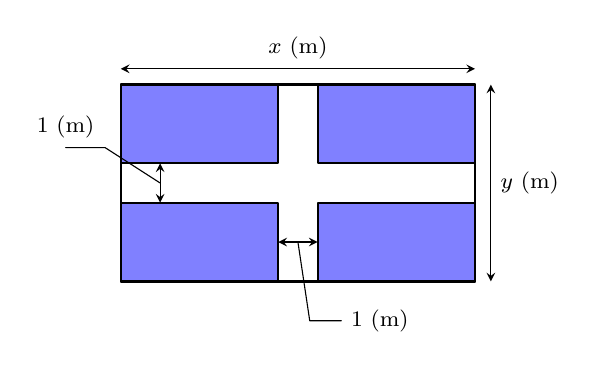
\begin{tikzpicture}[scale=1, font=\footnotesize, line join=round, line cap=round, >=stealth]
			\draw [fill=blue!50,thick] (0,0)--(2,0)--(2,1)--(0,1)--cycle;
			\draw [fill=blue!50,thick] (2.5,0)--(4.5,0)--(4.5,1)--(2.5,1)--cycle;
			\draw [fill=blue!50,thick] (0,1.5)--(2,1.5)--(2,2.5)--(0,2.5)--cycle;
			\draw [fill=blue!50,thick] (2.5,1.5)--(4.5,1.5)--(4.5,2.5)--(2.5,2.5)--cycle;
			\draw [thick](0,0)--(4.5,0)--(4.5,2.5)--(0,2.5)--cycle;
			\draw [<->](0,2.7)--(4.5,2.7) node[midway, above]{$x$ (m)};
			\draw [<->](4.7,0)--(4.7,2.5) node[midway, right]{$y$ (m)};
			\draw [<->] (0.5,1.5)--(0.5,1);
			\draw [<->] (2,0.5)--(2.5,0.5);
			\draw [thin] (0.5,1.25)--(-.2,1.7)--(-.7,1.7) node[above]{$1$ (m)};
			\draw [thin] (2.25,0.5)--(2.4,-.5)--(2.8,-.5) node[right]{$1$ (m)};
			%\node at (2.25,-1) {Hình 2};
		\end{tikzpicture}
	}
	\loigiai{
		\begin{enumerate}
			\item Phần còn lại của mảnh đất gồm bốn miếng đất bằng nhau có dạng hình chữ nhật với chiều dài bằng $\dfrac{x-1}{2}$ (m), chiều rộng bằng $\dfrac{y-1}{2}$ (m). Vậy đa thức biểu thị diện tích phần đất còn lại của mảnh đất đó là\\
			\[S=4\cdot\dfrac{x-1}{2}\cdot\dfrac{y-1}{2}=xy-x-y+1 \text{ (m$^2$)}.\]
			\item Thay $x=9$; $y=5{,}4$ vào $S$ ta được $S=9\cdot5{,}4-9-5{,}4+1=35{,}2 \text{ (m$^2$)}$.
		\end{enumerate}
	}
\end{vd}

\begin{vd}%[Dự án EX-9-Đề Cương Toán 8]%[Nguyễn Chiến]%[8D1H2-7]
	Từ một tấm tôn hình chữ nhật có chiều dài bằng $a$ (cm), chiều rộng bằng $b$ (cm), người ta cắt bỏ bốn hình vuông cạnh bằng $x$ (cm) ở bốn góc, rồi ráp và hàn thành thùng không có nắp (hình dưới).
	\begin{enumerate}
		\item  Viết biểu thức biểu thị thể tích nước tối đa mà thùng có thể chứa được.
		\item  Viết biểu thức biểu thị tổng diện tích năm mặt của chiếc thùng. 
		\item  Tính tổng diện tích năm mặt của chiếc thùng khi $a=9$ cm, $b=8$ cm và $x=3$ cm.
	\end{enumerate}
	\begin{center}
		\begin{tikzpicture}[scale=0.85, font=\footnotesize,>=stealth]
			\def\canhBC{4};\def\canhAB{3};
			\coordinate (B) at (0,0);
			\coordinate (A) at ($(B)+(90:\canhAB)$);
			\coordinate (C) at ($(B)+(0:\canhBC)$);
			\coordinate (D) at ($(A)+(0:\canhBC)$);
			\coordinate (I) at ($(B)!1!-90:(A)$);
			\coordinate (I) at ($(B)!1!-90:(A)$);
			\coordinate (J) at ($(C)!1!90:(D)$);
			\coordinate (K) at ($(D)!1!-90:(C)$);
			\coordinate (H) at ($(A)!1!90:(B)$);
			\coordinate (M) at ($(A)+1/5*(I)-1/5*(A)$);
			\coordinate (N) at ($(D)+1/5*(J)-1/5*(D)$);
			\coordinate (P) at ($(C)+1/5*(K)-1/5*(C)$);
			\coordinate (Q) at ($(B)+1/5*(H)-1/5*(B)$);
			\coordinate (S) at (intersection of M--N and A--B);
			\coordinate (W) at (intersection of M--N and D--C);
			\coordinate (E) at (intersection of M--Q and A--D);
			\coordinate (R) at (intersection of M--Q and B--C);
			\coordinate (T) at (intersection of Q--P and A--B);
			\coordinate (Y) at (intersection of Q--P and D--C);
			\coordinate (U) at (intersection of N--P and A--D);
			\coordinate (O) at (intersection of N--P and B--C);
			\draw (S)--(A)--(E) (U)--(D)--(W) (Y)--(C)--(O) (R)--(B)--(T);
			\draw [fill=cyan!20,thick](S)--(M)--(E)--(U)--(N)--(W)--(Y)--(P)--(O)--(R)--(Q)--(T)--cycle;
			\draw [dashed] (M)--(N)--(P)--(Q)--cycle;
			\draw[>=stealth,|<->|,transform canvas={shift={(-90:0.3)}}] (B)--(C) node[fill=white,inner sep=2pt,font=\scriptsize,midway,sloped]{$a$};
			\draw[>=stealth,|<->|,transform canvas={shift={(180:0.3)}}] (B)--(A) node[fill=white,inner sep=2pt,font=\scriptsize,midway,sloped]{$b$};
			\draw[>=stealth,|<->|,transform canvas={shift={(0:0.3)}}] (D)--(W) node[fill=white,inner sep=2pt,font=\scriptsize,midway,sloped]{$x$};
			%			\foreach \x/\y in {A/90, B/-90, C/-90, D/90,I/90,K/90,H/90,J/90,M/90,N/90,P/90,Q/90,S/90,W/90,E/90,R/90,T/90,U/90,O/90,Y/90}{\fill (\x) circle(1pt) ($(\x)+(\y:0.3cm)$) node{$\x$};}
		\end{tikzpicture}\hspace*{1cm}
		\begin{tikzpicture}[scale=0.8, font=\footnotesize,>=stealth]
			\def\canhAD{4};\def\canhBA{2};\def\gocBAD{-140};\def\h{0.7};\def\xdinhA'{0};
			\coordinate (A) at (0,0);
			\coordinate (B) at ($(A)+(\gocBAD:\canhBA)$);
			\coordinate (C) at ($(B)+(0:\canhAD)$);
			\coordinate (D) at ($(A)+(0:\canhAD)$);
			\coordinate (A') at ($(A)+(\xdinhA',\h)$);
			\coordinate (B') at ($(B)+(\xdinhA',\h)$);
			\coordinate (C') at ($(C)+(\xdinhA',\h)$);
			\coordinate (D') at ($(D)+(\xdinhA',\h)$);
			\coordinate (I) at (intersection of A--B and B'--C');
			\coordinate (K) at (intersection of A--D and D'--C');
			\draw [fill=cyan!20,thick](A')--(B')--(B)--(C)--(D)--(D')--cycle;
			\draw [thick](B')--(C')--(D') (C)--(C');
			\draw (A')--(A)--(I) (A)--(K);
			%			\foreach \x/\y in {A/180, B/180, C/0, D/0, A'/180, B'/180, C'/0, D'/0,I/90,K/90}{\fill (\x) circle(1pt) ($(\x)+(\y:0.3cm)$) node{$\x$};}
		\end{tikzpicture}
	\end{center}
	\loigiai{
		\begin{enumerate}
			\item 
			Thể tích nước tối đa mà thùng có thể chứa được là
			\[V=(a-2x)(b-2x)x=abx-2ax^2-2bx^2+4x^3 \text{ (cm$^3$).}\]
			\item 
			Tổng diện tích năm mặt của chiếc thùng là
			\[S=(a-2x)(b-2x)+2(b-2x)x+2(a-2x)x=ab-4x^2 \text{ (cm$^2$).}\]
			\item  Khi $a=9$ cm, $b=8$ cm và $x=3$ cm, tổng diện tích năm mặt của chiếc thùng là
			\[S=9 \cdot 8-4 \cdot 3^2=63 \text{ (cm$^2$).}\]
		\end{enumerate}
	}
\end{vd}
%%%%%%%%%%%%%%%%%%%%%%%%%%%%%%%%%%%%%%%%%%%%%%%%%%
\subsubsection{Bài tập}

\begin{bt}%[Dự án EX-9-Đề Cương Toán 8]%[Nguyễn Chiến]%[8D1H2-7]
		Bạn Chi dùng một miếng bìa hình chữ nhật có chiều dài $x$ (cm), chiều rộng $y$ (cm) (với $x>2$; $y>2$) để làm một chiếc hộp không nắp bằng cách cắt bốn hình vuông cạnh $1$ cm ở bốn góc rồi gấp lại. 
		\begin{enumerate}
			\item Viết đa thức biểu thị diện tích xung quanh (cm$^2$)  của chiếc hộp; 
			\item Viết đa thức biểu thị thể tích (cm$^3$) của chiếc hộp và tìm bậc của đa thức đó. 
			\item Tính thể tích của chiếc hộp khi $x=9$ cm và $y=5$ cm. 
		\end{enumerate}
	\begin{center}
		\begin{tikzpicture}[scale=0.85, font=\footnotesize,>=stealth]
			\def\canhBC{4};\def\canhAB{3};
			\coordinate (B) at (0,0);
			\coordinate (A) at ($(B)+(90:\canhAB)$);
			\coordinate (C) at ($(B)+(0:\canhBC)$);
			\coordinate (D) at ($(A)+(0:\canhBC)$);
			\coordinate (I) at ($(B)!1!-90:(A)$);
			\coordinate (I) at ($(B)!1!-90:(A)$);
			\coordinate (J) at ($(C)!1!90:(D)$);
			\coordinate (K) at ($(D)!1!-90:(C)$);
			\coordinate (H) at ($(A)!1!90:(B)$);
			\coordinate (M) at ($(A)+1/5*(I)-1/5*(A)$);
			\coordinate (N) at ($(D)+1/5*(J)-1/5*(D)$);
			\coordinate (P) at ($(C)+1/5*(K)-1/5*(C)$);
			\coordinate (Q) at ($(B)+1/5*(H)-1/5*(B)$);
			\coordinate (S) at (intersection of M--N and A--B);
			\coordinate (W) at (intersection of M--N and D--C);
			\coordinate (E) at (intersection of M--Q and A--D);
			\coordinate (R) at (intersection of M--Q and B--C);
			\coordinate (T) at (intersection of Q--P and A--B);
			\coordinate (Y) at (intersection of Q--P and D--C);
			\coordinate (U) at (intersection of N--P and A--D);
			\coordinate (O) at (intersection of N--P and B--C);
			\draw (S)--(A)--(E) (U)--(D)--(W) (Y)--(C)--(O) (R)--(B)--(T);
			\draw [fill=cyan!20,thick](S)--(M)--(E)--(U)--(N)--(W)--(Y)--(P)--(O)--(R)--(Q)--(T)--cycle;
			\draw [dashed] (M)--(N)--(P)--(Q)--cycle;
			\draw[>=stealth,|<->|,transform canvas={shift={(-90:0.3)}}] (B)--(C) node[fill=white,inner sep=2pt,font=\scriptsize,midway,sloped]{$x$};
			\draw[>=stealth,|<->|,transform canvas={shift={(180:0.3)}}] (B)--(A) node[fill=white,inner sep=2pt,font=\scriptsize,midway,sloped]{$y$};
			\draw[>=stealth,|<->|,transform canvas={shift={(0:0.3)}}] (D)--(W) node[fill=white,inner sep=2pt,font=\scriptsize,midway,sloped]{$1$};
			%			\foreach \x/\y in {A/90, B/-90, C/-90, D/90,I/90,K/90,H/90,J/90,M/90,N/90,P/90,Q/90,S/90,W/90,E/90,R/90,T/90,U/90,O/90,Y/90}{\fill (\x) circle(1pt) ($(\x)+(\y:0.3cm)$) node{$\x$};}
		\end{tikzpicture}\hspace*{1cm}
		\begin{tikzpicture}[scale=0.8, font=\footnotesize,>=stealth]
			\def\canhAD{4};\def\canhBA{2};\def\gocBAD{-140};\def\h{0.7};\def\xdinhA'{0};
			\coordinate (A) at (0,0);
			\coordinate (B) at ($(A)+(\gocBAD:\canhBA)$);
			\coordinate (C) at ($(B)+(0:\canhAD)$);
			\coordinate (D) at ($(A)+(0:\canhAD)$);
			\coordinate (A') at ($(A)+(\xdinhA',\h)$);
			\coordinate (B') at ($(B)+(\xdinhA',\h)$);
			\coordinate (C') at ($(C)+(\xdinhA',\h)$);
			\coordinate (D') at ($(D)+(\xdinhA',\h)$);
			\coordinate (I) at (intersection of A--B and B'--C');
			\coordinate (K) at (intersection of A--D and D'--C');
			\draw [fill=cyan!20,thick](A')--(B')--(B)--(C)--(D)--(D')--cycle;
			\draw [thick](B')--(C')--(D') (C)--(C');
			\draw (A')--(A)--(I) (A)--(K);
			%			\foreach \x/\y in {A/180, B/180, C/0, D/0, A'/180, B'/180, C'/0, D'/0,I/90,K/90}{\fill (\x) circle(1pt) ($(\x)+(\y:0.3cm)$) node{$\x$};}
		\end{tikzpicture}
	\end{center}
	\loigiai{
		\begin{enumerate}
			\item 
			Diện tích xung quanh của hộp giấy là
			\[S=(x-2+y-2) \cdot 2 \cdot 1=2x+2y-8 \text{ (cm$^2$).}\]
			\item 
			Thể tích của hộp giấy là
			\[V=(x-2)(y-2) \cdot 1=xy-2x-2y+4 \text{ (cm$^3$).}\]
			Bậc của đa thức này là $2$.
			\item Khi $x=9$ cm và $y=5$ cm thì thể tích của chiếc hộp là
			\[V=(9-2) \cdot (5-2) \cdot 1=21 \text{ (cm$^3$).}\]
		\end{enumerate}
	}
\end{bt}

\begin{bt}%[Dự án EX-9-Đề Cương Toán 8]%[Nguyễn Chiến]%[8D1H2-7]
	\immini{
		Khu vườn nhà bác An có dạng hình chữ nhật, chiều dài $x$ (m), chiều rộng $y$ (m). Bác định làm lối đi xung quanh vườn rộng $1$ m, phần còn lại để trồng rau.  
		\begin{enumerate}
			\item Viết đa thức biểu thị diện tích (m$^2$) để trồng rau;  
			\item Viết đa thức biểu thị diện tích (m$^2$) làm lối đi.
			\item Với $x=12$; $y=9$, tính diện tích làm lối đi.
		\end{enumerate}
	}
	{
		\begin{tikzpicture}[font=\footnotesize,line join=round, line cap=round, >=stealth,scale=0.8] 
			\foreach \x/\y/\pos in {0/0/A, 6/0/B, 0/4.5/D} \path ($(\x,\y)$) coordinate (\pos); 
			\path ($(B)+(D)-(A)$) coordinate (C)
			($(A)+(45:1)$) coordinate (M)
			($(B)+(135:1)$) coordinate (N)
			($(C)+(-135:1)$) coordinate (P)
			($(D)+(-45:1)$) coordinate (Q);
			\draw[<->] ($(A)!1/2!(D)$)--($(M)!1/2!(Q)$) node[pos=0.5,above]{$1$ m};
			\draw[<->] ($(A)!1/2!(B)$)--($(M)!1/2!(N)$) node[pos=0.5,right]{$1$ m};
			\draw[<->] ($(B)!1/2!(C)$)--($(N)!1/2!(P)$) node[pos=0.5,above]{$1$ m};
			\draw[<->] ($(C)!1/2!(D)$)--($(P)!1/2!(Q)$) node[pos=0.5,right]{$1$ m};
			\fill[green!30] (M)--(N)--(P)--(Q)--(M);
			\node[inner sep=3pt, fill=white] at ($(A)!1/2!(C)$){\text{Vườn rau}};
			\draw (A)--(B)--(C)--(D)--(A) (M)--(N)--(P)--(Q)--(M);
		\end{tikzpicture}
	}
	\loigiai{
	\begin{enumerate}
		\item Đa thức biểu thị diện tích để trồng rau là 
		\[S=(x-2)(y-2)=xy-2x-2y+4 \text{ (m$^2$).}\]
		\item Đa thức biểu thị diện tích làm lối đi là
		\[S=xy-(xy-2x-2y+4)=2x+2y-4\text{ (m$^2$).}\]
		\item Với $x=12$; $y=9$, diện tích làm lối đi là
		\[S=2\cdot 12+2\cdot 9-4=38 \text{ (m$^2$).}\]
	\end{enumerate}
	}
\end{bt}

\begin{bt}%[Dự án EX-9-Đề Cương Toán 8]%[Nguyễn Chiến]%[8D1H2-7]
	Một khu vườn hình vuông có độ dài cạnh bằng $2x$ (m). Người ta làm đường đi xung quanh khu vườn, có độ rộng như nhau và bằng $y$ (m) với $x>2y$.
	\begin{enumerate}
		\item Viết biểu thức biểu thị diện tích $S$ (m$^2$) của đường đi bao quanh mảnh vườn theo $x$ và $y$.
		\item Tính $S$ khi $x=11$, $y=0{,}5$.
	\end{enumerate}
	\loigiai{
		\begin{enumerate}
			\item Biểu thức biểu thị diện tích của đường đi bao quanh mảnh vườn là
			\[S=(2x)^2-(x-2y)^2=3x^2+4xy-4y^2 \text{ (m$^2$).}\]
			\item Thay $x=11$, $y=0{,}5$ vào $S$ ta được
			\[S=3\cdot 11^2+4\cdot 11\cdot 0{,}5-4\cdot 0{,}5^2=384 \text{ (m$^2$).}\]
		\end{enumerate}
	}
\end{bt}

\begin{bt}%[Dự án EX-9-Đề Cương Toán 8]%[Nguyễn Chiến]%[8D1H2-7]
	Một tấm bìa hình chữ nhật có diện tích bằng $6xy+10y^2$ (cm) và chiều rộng bằng $2y$ (cm).
	\begin{enumerate}
		\item Viết biểu thức biểu thị chiều dài của tấm bìa.
		\item Viết biểu thức biểu thị chu vi của tấm bìa.
		\item Cho $x=3$ và $y=4$, tính chu vi của tấm bìa.
	\end{enumerate}
	\loigiai{
		\begin{enumerate}
			\item Biểu thức biểu thị chiều dài của tấm bìa là
			\[(6xy+10y^2):(2y)=3x+5y \text{ (cm).}\]
			\item Viết biểu thức biểu thị chu vi của tấm bìa là
			\[(3x+5y+2y) \cdot 2=6x+14y \text{ (cm).}\]
			\item Với $x=3$ và $y=4$ thì chu vi của tấm bìa là
			\[6\cdot 3+14\cdot 4=74 \text{ (cm).}\]
		\end{enumerate}
	}
\end{bt}

\begin{bt}%[Dự án EX-9-Đề Cương Toán 8]%[Nguyễn Chiến]%[8D1H2-7]
	Một sân chơi hình chữ nhật có chu vi bằng $4x+8y$ (m) và chiều rộng bằng $x-y$ (m) với $x>y$.
	\begin{enumerate}
		\item Viết biểu thức biểu thị chiều dài của sân chơi.
		\item Viết biểu thức biểu thị diện tích của sân chơi.
		\item Cho $x=4$ và $y=1$, tính diện tích của sân chơi.
	\end{enumerate}
	\loigiai{
		\begin{enumerate}
			\item Biểu thức biểu thị chiều dài của sân chơi là
			\[(4x+8y):2-(x-y)=x+5y \text{ (m).}\]
			\item Biểu thức biểu thị diện tích của sân chơi là
			\[(x+5y)(x-y)=x^2+4xy-5y^2 \text{ (m$^2$).}\]
			\item Khi $x=4$ và $y=1$ thì diện tích của sân chơi là
			\[4^2+4\cdot 4\cdot 1-5\cdot 1^2=27 \text{ (m$^2$).}\]
		\end{enumerate}
	}
\end{bt}

\begin{bt}%[Dự án EX-9-Đề Cương Toán 8]%[Nguyễn Chiến]%[8D1H2-7]
	Một sân vận động hình chữ nhật có chiều dài $5x+3y$ (m) và chiều rộng là $5x-3y$ (m). Người ta làm lối đi xung quanh sân vận động, độ rộng của lối đi là $3$ m, phần trong là phần sân trồng cỏ phục vụ cho các trận bóng đá.
	\begin{enumerate}
		\item Viết biểu thức biểu thị diện tích mặt sân có trồng cỏ theo $x$ và $y$.
		\item Tính số tiền trồng cỏ cho mặt sân trên khi $x=10$, $y=2$. Biết số tiền để trồng $1$ m$^2$ cỏ là $50\,000$ đồng.
	\end{enumerate}
	\loigiai{
		\begin{enumerate}
			\item Biểu thức biểu thị diện tích mặt sân có trồng cỏ theo $x$ và $y$ là 
			\[S=(5x+3y-6)(5x-3y-6)=25x^2-60x-9y^2+36 \text{ (m$^2$).}\]
			\item Khi $x=10$, $y=2$ thì diện tích mặt sân có trồng cỏ là
			\[S=25\cdot10^2-60\cdot10-9\cdot2^2+36=1\,900 \text{ (m$^2$).}\]
			Số tiền trồng cỏ cho mặt sân trên là
			\[50\,000\cdot 1\,900= 95\,000\,000 \text{ (đồng).}\]
		\end{enumerate}
	}
\end{bt}

\begin{bt}%[Dự án EX-9-Đề Cương Toán 8]%[Nguyễn Chiến]%[8D1H2-7]
	Bác Hòa mua tôn về để gò một hình lăng trụ đứng (rỗng hai đáy) có đáy là tam giác đều cạnh $(2x-y)$ (dm), chiều cao $(4x-3y)$ (dm). 
	\begin{enumerate}
		\item Viết biểu thức biểu thị diện tích xung quanh của hình lăng trụ đứng đó.
		\item Biết rằng $x=3$; $y=2$ và giá mỗi dm$^2$ tôn là $25\,000$ đồng. Tính tổng số tiền bác Hòa cần mua tôn.
	\end{enumerate}
	\loigiai{
		\begin{enumerate}
			\item Biểu thức biểu thị diện tích xung quanh của hình lăng trụ đứng đó là
			\[S=3(2x-y)(4x-3y)=24x^2-30xy+9y^2 \text{ (dm$^2$).}\]
			\item Khi $x=3$, $y=2$ thì diện tích tôn cần mua là
			\[S=24\cdot 3^2-30\cdot 3 \cdot 2+9\cdot 2^2=72 \text{ (dm$^2$).}\]
			Số tiền bác Hòa cần mua tôn là
			\[25\,000  \cdot 72= 1\,800\,000 \text{ (đồng).}\]
		\end{enumerate}
	}
\end{bt}

\begin{bt}%[Dự án EX-9-Đề Cương Toán 8]%[Nguyễn Chiến]%[8D1H2-7]
	Mỗi quyển vở giá $x$ (đồng), mỗi cái bút giá $y$ (đồng).
	\begin{enumerate}
		\item Viết biểu thức biểu thị số tiền phải trả để mua $40$ quyển vở và $10$ cái bút.
		\item Tính số tiền phải trả để mua $40$ quyển vở và $10$ cái bút biết giá 1 quyển vở là $7\,000$ đồng và giá $1$ cái bút là $5\,000$ đồng.
	\end{enumerate}
	\loigiai{
		\begin{enumerate}
			\item Biểu thức biểu thị số tiền phải trả để mua $40$ quyển vở và $10$ cái bút là 
			\[40x+10y \text{ (đồng).}\]
			\item Số tiền phải trả để mua $40$ quyển vở và $10$ cái bút  đó là
			\[40\cdot 7\,000+10\cdot 5\,000=330\,000 \text{ (đồng).}\]
		\end{enumerate}
	}
\end{bt}

\begin{bt}%[Dự án EX-9-Đề Cương Toán 8]%[Nguyễn Chiến]%[8D1H2-7]
	\immini{
		Một hộp giấy có dạng hình hộp chữ nhật với chiều rộng là $x$ (cm), chiều dài hơn chiều rộng $y$ (cm) và chiều cao là $y+2$ (cm) \textit{(Hình bên)}. 
		\begin{enumerate}
			\item Viết đa thức biểu thị thể tích của hộp giấy đó.
			\item Viết đa thức biểu thị tổng diện tích các mặt của hộp giấy đó.
			\item Cho $x=8$ và $y=5$. Tính tổng diện tích các mặt của hộp giấy đó.
		\end{enumerate}
	}
	{
		\begin{tikzpicture}[scale=1, font=\footnotesize, line join=round, line cap=round, >=stealth]
			\def\a{4}
			\def\b{1}
			\def\h{2}
			\path 	(0:0) coordinate (A)
			++(0:\a) coordinate (D)
			++(-130:\b) coordinate (C)
			($(A)+(C)-(D)$) coordinate (B)
			($(A)+(90:\h)$) coordinate (A')
			($(B)+(90:\h)$) coordinate (B')
			($(C)+(90:\h)$) coordinate (C')
			($(D)+(90:\h)$) coordinate (D');
			\draw[dashed,thick] 	(B)--(A)--(D)	(A)--(A');
			\draw[thick] 	(C)--(C') 	(D)--(D') node[midway, below, rotate=90]{$y+2$ (cm)}	(B)--(B')	(C)--(C')
			(B)--(C) node[midway, below]{$x+y$ (cm)}--(D)node[midway, below, rotate=50]{$x$ (cm)} 
			(A')--(B')--(C')--(D')--cycle;
			%\path ($(B)!.5!(C)$)--++(-90:.6) node[below]{Hình 1};
		\end{tikzpicture}
	}
	\loigiai{
		\begin{enumerate}
			\item Chiều dài của hộp giấy đó là $x+y$ (cm).\\
				Đa thức biểu thị thể tích của hộp giấy đó là 
				\[V=x(x+y)(y+2)=x^2y+2x^2+xy^2+2xy \text{ (cm$^3$).}\]
			\item Đa thức biểu thị tổng diện tích các mặt của hộp giấy đó là
			\allowdisplaybreaks
			\begin{eqnarray*}
			   S&=&2[x(x+y)+(x+y)(y+2)+(y+2)x]\\ 
				&=& 2(x^2+xy+xy+2x+y^2+2y+xy+2x)\\
				&=& 2(x^2+3xy+4x+y^2+2y)\\
				&=& 2x^2+6xy+8x+2y^2+4y \text{ (cm$^2$).}
			\end{eqnarray*}
			\item Cho $x=8$ và $y=5$. Tính tổng diện tích các mặt của hộp giấy đó là 
				\[S=2 \cdot 8^2+6 \cdot 8 \cdot 5+8 \cdot 8+2 \cdot 5^2+4 \cdot 5=502 \text{ (cm$^2$).}\]
		\end{enumerate}
	}
\end{bt}

\begin{bt}%[Dự án EX-9-Đề Cương Toán 8]%[Nguyễn Chiến]%[8D1H2-7]
	Từ tỉnh $A$ một người đi xe máy với tốc độ $v$ (km/h) trong $3$ giờ đầu, sau đó xe đi với tốc độ gấp rưỡi tốc độ trước đó trong $t$ giờ thì đến tỉnh $B$. Một người khác đi xe đạp từ tỉnh $A$ đến tỉnh $B$ với tốc độ bằng $\dfrac{1}{3}$ tốc độ ban đầu của xe máy. 
	\begin{enumerate}
		\item Viết biểu thức tính quãng đường $AB$ theo $v$ và $t$.
		\item Viết biểu thức tính thời gian xe đạp đi hết quãng đường $AB$.
	\end{enumerate}
	\loigiai{
		\begin{enumerate}
			\item Biểu thức tính quãng đường $AB$ theo $v$ và $t$ là
			\[3v+\dfrac{3}{2}vt \text{ (km).}\]
			\item Vận tốc của xe đạp là $\dfrac{1}{3}v$ (km/h).\\
			Thời gian xe đạp đi hết quãng đường $AB$ là
			\[\left(3v+\dfrac{3}{2}vt\right):\left(\dfrac{1}{3}v\right)=9+\dfrac{9}{2}t \text{ (giờ).}\]
		\end{enumerate}
	}
\end{bt}

\begin{bt}%[Dự án EX-9-Đề Cương Toán 8]%[Nguyễn Chiến]%[8D1H2-7]
	Một hộp giấy dạng hình hộp chữ nhật có chiều dài là $5x$ (dm), chiều rộng là $4y$ (dm) và thể tích là $40x^2y^2$ (dm$^3$).
	\begin{enumerate}
		\item Viết biểu thức biểu thị chiều cao của hộp giấy.
		\item Người ta sơn bốn mặt xung quanh của hộp giấy. Viết biểu thức biểu thị diện tích cần sơn.
		\item Với $x=1$ và $y=0{,}5$, tính diện tích cần sơn.
	\end{enumerate}
	\loigiai{
		\begin{enumerate}
			\item Biểu thức biểu thị chiều cao của hộp giấy là
			\[40x^2y^2:(5x \cdot 4y)=2xy \text{ (dm).}\]
			\item Biểu thức biểu thị diện tích cần sơn là
			\[\left(5x+4y\right) \cdot 2 \cdot 2xy=20x^2y+16xy^2 \text{ (dm$^2$).}\]
			\item Với $x=1$ và $y=0{,}5$ thì diện tích cần sơn là
			\[20\cdot 1^2\cdot 0{,}5+16\cdot 1\cdot 0{,}5^2=14 \text{ (dm$^2$).}\]
		\end{enumerate}
	}
\end{bt}

\begin{bt}%[Dự án EX-9-Đề Cương Toán 8]%[Nguyễn Chiến]%[8D1H2-7]
	Một khối gỗ hình lăng trụ đứng tam giác đều có thể tích $5x^2y-4xy^2$ (cm$^3$) và chiều cao  là $3xy$ (cm).
	\begin{enumerate}
		\item Viết biểu thức biểu thị diện tích đáy của khối gỗ.
		\item Với $x=3$ và $y=1{,}5$, tính diện tích đáy của khối gỗ.
	\end{enumerate}
	\loigiai{
		\begin{enumerate}
			\item Biểu thức biểu thị diện tích đáy của khối gỗ là
			\[3\left(5x^2y-4xy^2\right):(3xy)=5x-4y \text{ (cm$^2$).}\]
			\item Với $x=3$ và $y=1{,}5$ thì diện tích cần sơn là
			\[5\cdot 3-4\cdot 1{,}5=9 \text{ (cm$^2$).}\]
		\end{enumerate}
	}
\end{bt}